\documentclass{beamer}
\usepackage{ctex}
\usepackage{makecell}
\usepackage{amsmath}
\usepackage{array}
\usepackage{graphicx}
\usepackage{pdfpages}
\usepackage{float}
\usepackage{fancyhdr}
\usepackage{multirow}
\usepackage{diagbox}
\usepackage{siunitx}
\usepackage{verbatim}
\usepackage{indentfirst}
\usepackage{caption}
\usepackage{circuitikz}
\usepackage{subfigure}
\usepackage{tikz}
\usepackage{pgfkeys}
\usepackage{pgffor}
\usepackage{pgfcalendar}
\usepackage{pgfpages}
\usepackage{booktabs}
\usepackage{diagbox}
\usetikzlibrary{calc,angles,positioning,intersections,arrows.meta}
\setlength{\parindent}{2em}
\title{My Recent Work}
\author{Qian Sitian}
\date{2018/7/25}
\begin{document}
%\maketitle
\begin{frame}
    \titlepage
\end{frame}
\begin{frame}
    \frametitle{Outline}
    \tableofcontents
\end{frame}
\begin{frame}   
    \section{Parameter Fitting}
    \frametitle{Parameter Fitting}
    \begin{itemize}
        \item Preview
        \item Parameters to Obserables
        \item Obserables to Parameters
    \end{itemize}
\end{frame}\
\begin{frame}{Preview}
    \subsection{Preview}
    \begin{itemize}
        \item Basic Information
        \item Target
        \item Data
    \end{itemize}
\end{frame}
\begin{frame}
    \frametitle{Basic Information}
    
    Basic Information
    \begin{itemize}
        \item Model:\\Collective 
        ow in 2.76 A TeV and 5.02 A TeV Pb+Pb
        collisions
        \\
        Arxiv:1703.10792
        \item Motivation:\\Applying Bayesian parameter estimation to relativistic heavy-ion collisions:
        simultaneous characterization of the initial state and quark-gluon plasma medium
        \\
        Arxiv:1605.03954
    \end{itemize}
\end{frame}
\begin{frame}
    \frametitle{Target}
    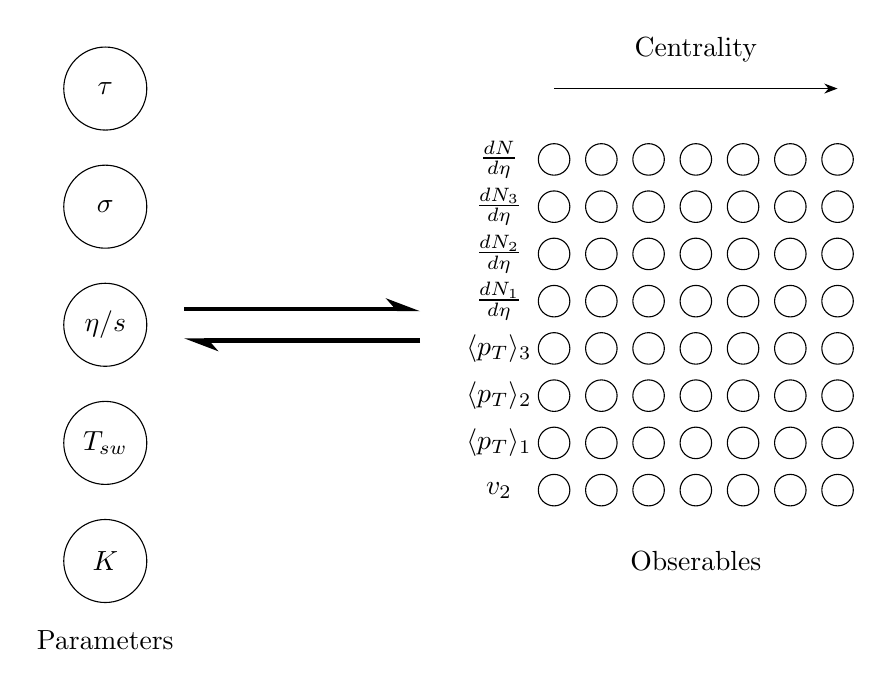
\begin{tikzpicture}
        \node[circle,draw] at (0,3+4)[minimum size=30pt] {$\tau$};
        \node [circle,draw]at (0,1.5+4)[minimum size=30pt] {$\sigma$};
        \node [circle,draw]at (0,0+4)[minimum size=30pt] {$\eta/s$};
        \node [circle,draw]at (0,-1.5+4)[minimum size=30pt] {$T_{sw}$};
        \node [circle,draw]at (0,-3+4)[minimum size=30pt] {$K$};
        \node at(0,-4+4){Parameters};
        \draw [arrows = {-Stealth[harpoon]},ultra thick] (1,4.2) -- (4,4.2);
        \draw [arrows = {-Stealth[harpoon]},ultra thick] (4,3.8) -- (1,3.8);
        \foreach \x in{0,1,2,3,4,5,6,7} \foreach \y in {0,1,2,3,4,5,6}
            \draw  (7.5+0.6*\y-1.8,4+0.6*\x-2.1) circle(0.2cm);
        \foreach \name/\x in{v_2/0,\langle p_T\rangle_1/1,\langle p_T\rangle_2/2,\langle p_T\rangle_3/3,\frac{dN_1}{d\eta}/4,\frac{dN_2}{d\eta}/5,\frac{dN_3}{d\eta}/6,\frac{dN}{d\eta}/7}
            \node at (5,4+0.6*\x-2.1) {$\name$};
        \node at(7.5,-3+4){Obserables};
        \node at(7.5,3.5+4){Centrality};
        \draw [{arrows = {-Stealth[reversed, reversed]}},] (7.5-1.8,7) -- (7.5+1.8,7);
    \end{tikzpicture}
\end{frame}
\begin{frame}
    \frametitle{Data}
    \begin{itemize}
        \item Initial:
 
        \begin{table}
            \centering
            \begin{tabular}{c|c|c|c|c}
                \toprule
                $\tau$&$\sigma$&$\eta/s$&$T_{sw}$&$K$\\
                \midrule
                0.2&0.2&0.02&0.15&0.4\\
                0.6&0.6&0.08&0.24&0.8\\
                0.9&1.0&0.12&0.4&1.2\\
                \bottomrule
            \end{tabular}
        \end{table}
    \item Divide:

    $$ Total:3^5=243\Rightarrow\left\{
\begin{aligned}
Train:& 220 \\
Test:& 23
\end{aligned}
\right.
$$
    \end{itemize}
    
\end{frame}
\begin{frame}
    \subsection{Parameters to Obserables}
    \frametitle{Parameters to Obserables}
    \begin{itemize}
        \item Network
        \item Result
    \end{itemize}
\end{frame}
\begin{frame}
    \frametitle{Network}
    \begin{itemize}
        \item Optimizer:Adam
        \item Learning rate:0.0005
        \item Loss:The L2 norm of the absolute error between the predictions and the labels 
        \item Batch size:Randomly choose 44 of 220
        \item Layers' type:FC with dropout(p=0.5),activation function:relu
        \item Training times:200000
    \end{itemize}
    

\end{frame}
\begin{frame}{Network}
    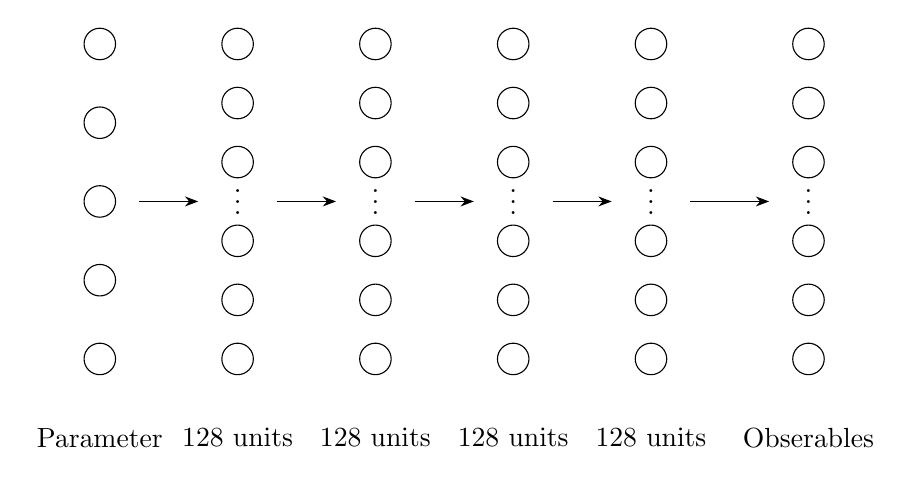
\begin{tikzpicture}
        \foreach \x in {0,1,2,3,4}
            \draw (0,\x) circle(0.2cm);
        \node at (0,-1) {Parameter};
        \draw [{arrows = {-Stealth[reversed, reversed]}}] (0.5,2) -- (1.25,2);
        \foreach \x in {0,1,2}
            {\draw (1.75,2+0.5+\x*0.75) circle(0.2cm); \draw (1.75,2-0.5-\x*0.75) circle(0.2cm);}
        \node at (1.75,2+0.1){$\vdots$};
        \node at (1.75,-1){128 units};
        \draw [{arrows = {-Stealth[reversed, reversed]}}] (2.25,2) -- (3,2);
        \foreach \x in {0,1,2}
            {\draw (3.5,2+0.5+\x*0.75) circle(0.2cm); \draw (3.5,2-0.5-\x*0.75) circle(0.2cm);}
        \node at (3.5,2+0.1){$\vdots$};
        \node at (3.5,-1){128 units};
        \draw [{arrows = {-Stealth[reversed, reversed]}}] (4,2) -- (4.75,2);
        \foreach \x in {0,1,2}
            {\draw (5.25,2+0.5+\x*0.75) circle(0.2cm); \draw (6-0.75,2-0.5-\x*0.75) circle(0.2cm);}
        \node at (6-0.75,2+0.1){$\vdots$};
        \node at (6-0.75,-1){128 units};
        \draw [{arrows = {-Stealth[reversed, reversed]}}] (6.5-0.75,2) -- (6.5,2);
        \foreach \x in {0,1,2}
            {\draw (7,2+0.5+\x*0.75) circle(0.2cm); \draw (7,2-0.5-\x*0.75) circle(0.2cm);}
        \node at (7,2+0.1){$\vdots$};
        \node at (7,-1){128 units};
        \draw [{arrows = {-Stealth[reversed, reversed]}}] (7.5,2) -- (8.5,2);
        \foreach \x in {0,1,2}
            {\draw (9,2+0.5+\x*0.75) circle(0.2cm); \draw (9,2-0.5-\x*0.75) circle(0.2cm);}
        \node at (9,2+0.1){$\vdots$};
        \node at (9,-1){Obserables};
    \end{tikzpicture}
\end{frame}
\begin{frame}
    \frametitle{Result}
    \begin{figure}[H]
    \includegraphics[width=\textwidth]{Result1.jpg}
    %\caption{Result}
    \label{fig:}
    \end{figure}
\end{frame}
\begin{frame}{Result:Relative Error}
% Table generated by Excel2LaTeX from sheet 'Sheet4'
\begin{table}[htbp]
    \centering
    \caption{Relative Error}
      \begin{tabular}{c|c|c|c|c|c|c|c}
        \toprule
      \diagbox[width=4em,trim=l]{Obs}{Ctr} & 2.5\% &7.5\% & 15\% & 25\% & 35\% &45\% &55\%\\
      \midrule
      $\frac{dN}{d\eta}$ & 0.01  & 0.01  & 0.01  & 0.01  & 0.02  & 0.02  & 0.04 \\
      $\frac{dN_1}{d\eta}$ & 0.02  & 0.02  & 0.03  & 0.03  & 0.03  & 0.05  & 0.05 \\
      $\langle p_T\rangle_1$ & 0.04  & 0.02  & 0.04  & 0.04  & 0.06  & 0.05  & 0.05 \\
      $\langle p_T\rangle_2$ & 0.04  & 0.05  & 0.03  & 0.03  & 0.05  & 0.04  & 0.04 \\
      $\langle p_T\rangle_3$ & 0.02  & 0.08  & 0.03  & 0.04  & 0.09  & 0.10  & 0.16 \\
      $\frac{dN_2}{d\eta}$ & 0.01  & 0.01  & 0.01  & 0.01  & 0.02  & 0.02  & 0.04 \\
      $\frac{dN_3}{d\eta}$ & 0.03  & 0.05  & 0.04  & 0.04  & 0.06  & 0.07  & 0.13 \\
      $v_2$ & 1.17  & 1.34  & 0.63  & 0.72  & 0.94  & 0.36  & 1.18 \\
      \bottomrule
      \end{tabular}%
    \label{tab:addlabel}%
  \end{table}%
  
\end{frame}
\begin{frame}
    \subsection{Obserables to Parameters}
    \frametitle{Obserables to Parameters}
    \begin{itemize}
        \item Network
        \item Result
    \end{itemize}
\end{frame}
\begin{frame}
    \frametitle{Network}
    \begin{itemize}
        \item Optimizer:Adam
        \item Learning rate:0.0005
        \item Loss:The L2 norm of the absolute error between the predictions and the labels 
        \item Batch size:Randomly choose 44 of 220
        \item Layers' type:FC with dropout(p=0.5),activation function:relu
        \item Training times:200000
    \end{itemize}
    

\end{frame}
\begin{frame}{Network}
    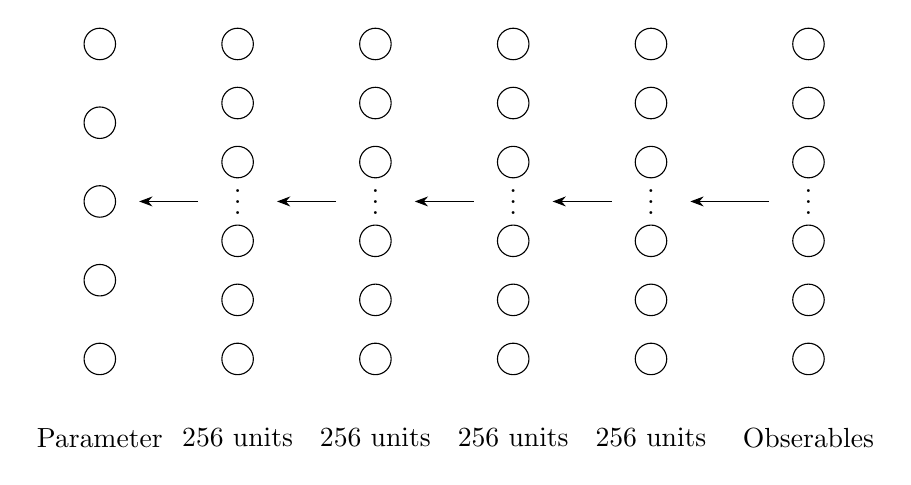
\begin{tikzpicture}
        \foreach \x in {0,1,2,3,4}
            \draw (0,\x) circle(0.2cm);
        \node at (0,-1) {Parameter};
        \draw [{arrows = {-Stealth[reversed, reversed]}}] (1.25,2) -- (0.5,2);
        \foreach \x in {0,1,2}
            {\draw (1.75,2+0.5+\x*0.75) circle(0.2cm); \draw (1.75,2-0.5-\x*0.75) circle(0.2cm);}
        \node at (1.75,2+0.1){$\vdots$};
        \node at (1.75,-1){256 units};
        \draw [{arrows = {-Stealth[reversed, reversed]}}] (3,2) -- (2.25,2);
        \foreach \x in {0,1,2}
            {\draw (3.5,2+0.5+\x*0.75) circle(0.2cm); \draw (3.5,2-0.5-\x*0.75) circle(0.2cm);}
        \node at (3.5,2+0.1){$\vdots$};
        \node at (3.5,-1){256 units};
        \draw [{arrows = {-Stealth[reversed, reversed]}}] (4.75,2) -- (4,2);
        \foreach \x in {0,1,2}
            {\draw (5.25,2+0.5+\x*0.75) circle(0.2cm); \draw (6-0.75,2-0.5-\x*0.75) circle(0.2cm);}
        \node at (6-0.75,2+0.1){$\vdots$};
        \node at (6-0.75,-1){256 units};
        \draw [{arrows = {-Stealth[reversed, reversed]}}] (6.5,2) -- (6.5-0.75,2);
        \foreach \x in {0,1,2}
            {\draw (7,2+0.5+\x*0.75) circle(0.2cm); \draw (7,2-0.5-\x*0.75) circle(0.2cm);}
        \node at (7,2+0.1){$\vdots$};
        \node at (7,-1){256 units};
        \draw [{arrows = {-Stealth[reversed, reversed]}}] (8.5,2) -- (7.5,2);
        \foreach \x in {0,1,2}
            {\draw (9,2+0.5+\x*0.75) circle(0.2cm); \draw (9,2-0.5-\x*0.75) circle(0.2cm);}
        \node at (9,2+0.1){$\vdots$};
        \node at (9,-1){Obserables};
    \end{tikzpicture}
\end{frame}

\begin{frame}{Result:Relative Error}
% Table generated by Excel2LaTeX from sheet 'Sheet4'
\begin{table}[htbp]
    \centering
    \caption{Relative Rrror}
      \begin{tabular}{c|c|c|c|c}\toprule
      $\tau$ & $\sigma$ & $\eta/s$ & $T_{sw}$ & $K$ \\\midrule
      0.053011 & 0.201948 & 1.538553 & 0.065286 & 0.059904 \\\bottomrule
      \end{tabular}%
    \label{tab:addlabel}%
  \end{table}%
  
\end{frame}
\begin{frame}
    \section{Reinforcement Learning}
    \frametitle{Reinforcement Learning}
    Studying something basic like Boltzmann's Equation, Fluid Mechanics...


\end{frame}
\begin{frame}
    Thank you for listening!
\end{frame}
\end{document}